\chapter{Related work}
\label{ch:Related-Work}
This chapter introduces and explains terms and concepts used throughout the thesis. Thus, this section can be used as a reference guide to fill in any gaps and to understand the relationships between the individual concepts better.

\section{Introduction to digital signal processing}
\label{sec:Intro-DSP}
This section introduces the fundamentals of \gls{DSP}, which will be used repeatedly in the following sections, either to describe some behaviour or to reason. 
\newline
\newline
What exactly is \gls{DSP}? \gls{DSP} is to take real-world signals like voice, audio, video, temperature, pressure, or position that have been digitized and mathematically manipulate them. A \gls{DSP} is designed for performing mathematical functions such as \textit{add}, \textit{subtract}, \textit{multiply} and \textit{divide} very quickly.
\newline
\newline
Signals need to be processed so that the information that they contain can be displayed, analyzed, or converted to another type of signal that may be of use. In the real-world, analogue products detect signals such as sound, light, temperature or pressure and manipulate them. Converters such as an \gls{ADC} then take the real-world signal and turn it into the digital format of \texttt{1}'s and \texttt{0}'s. From here, the \gls{DSP} takes over by capturing the digitized information and processing it. It then feeds the digitized information back for use in the real world. It does this in one of two ways, either digitally or in an analogue format by going through a \gls{DAC}. All of this occurs at very high speed.\footnotemark
\footnotetext{\href{https://www.analog.com/en/design-center/landing-pages/001/beginners-guide-to-dsp.html}{analog.com/en/design-center/landing-pages/001/beginners-guide-to-dsp.html}}

\subsection{Waveform}
\label{sub:Waveform}
Speech signals are sound signals, which are defined as pressure variations travelling through the air. These variations in pressure can be described as waves, and are therefore often called sound waves. In the current thesis, the focus is on the analysis and processing of such waveforms in digital systems. Therefore it is always assumed that the acoustic speech signals have been captured by a microphone and converted to a digital form.
\newline
\newline
A speech signal of finite length can be represented by a digitalised finite-length sequence $x[n]$, with $n = 0, 1, \dots, N-1$.

\subsection{Amplitude}
\label{sub:Amplitude}
The amplitude of a periodic variable is the measure of how far, and in what direction, that variable differs from zero. Thus, signal amplitudes can be either positive or negative. If the amplitude of a given signal is large, the signal is observed to be loud. Equation \ref{eq:Wave-Equation} shows a simple form of a wave equation, where $y$ is the oscillating variable (signal), $A$ the amplitude, $\gamma$ the period, $t$ the time and $\phi$ the phase shift. $sin(t)$ has a period of $2 \phi$. Figure \ref{fig:Amplitude-Wavelenght} illustrates such a simple wave form. 
\myequations{Simple wave equation}
\begin{equation}
    \centering
    y(t) = A \ sin(\gamma \ t + \phi)
    \label{eq:Wave-Equation}
\end{equation}
The distance from the top of one peak to the bottom of another is called the \textit{peak-to-peak amplitude}. Another way to describe peak-to-peak amplitude is to say that it is the distance between the maximum value and the minimum value of a wave. In figure \ref{fig:Amplitude-Wavelenght}, the peak-to-peak amplitude of the wave would be $2A$.

\subsection{Magnitude}
\label{sub:Magnitude}
The magnitude of a periodic variable is the measure of how far, regardless of direction, its quantity differs from zero. So magnitudes are always positive values. Occasionally, in the literature of digital signal processing, the term magnitude is referred to as the absolute value. In figure \ref{fig:Amplitude-Wavelenght}, the magnitude of the wave would be $|A|$.

\subsection{Period}
\label{sub:Period}
The period is the length of a single cycle of a wave, as measured by the distance between one peak of a wave and the next. In figure \ref{fig:Amplitude-Wavelenght}, the wavelength is denoted as the variable $\gamma$. But not every signal is periodic, only if the signal satisfies the condition $\gamma = 2k\pi$ where $k \in \mathbb{Z}$.

\subsection{Frequency}
\label{sub:Frequency}
Frequency is the number of occurrences of a repeating event per unit of time. It depends on the wavelength of an audio signal $\lambda$. The frequency is given by the equation \ref{eq:Frequency}. If the signal at a given time has a high frequency, it is observed to have a higher pitch.

\myequations{Calculate frequency from wavelength}
\begin{equation}
    \centering
    f = \frac{1}{\gamma}
    \label{eq:Frequency}
\end{equation}

% TODO change image to notation used in equation!
\begin{figure}[htbp]
	\centering
	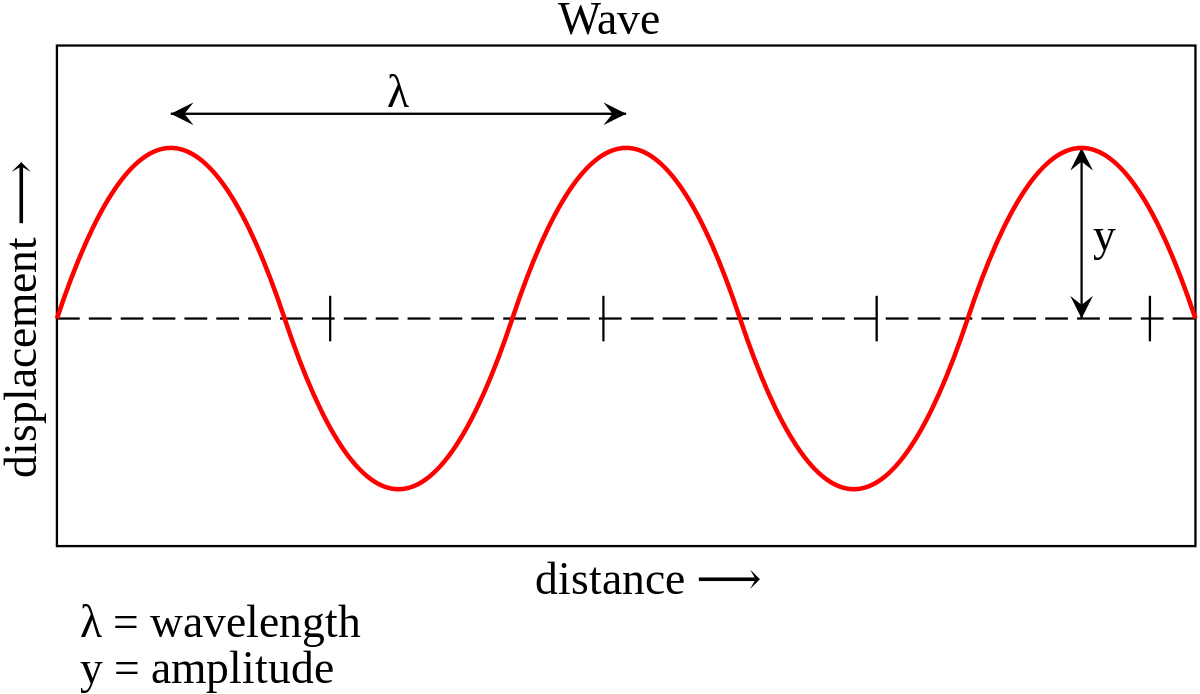
\includegraphics[scale=0.25]{img/Amplitude.png}
	\caption[Amplitude and wavelength illustrated]{Amplitude and wavelength \footnotemark}
	\label{fig:Amplitude-Wavelenght}
\end{figure}
\footnotetext{\href{https://en.wikiversity.org/wiki/Amplitude}{\nolinkurl{en.wikiversity.org/wiki/Amplitude}}}

\subsection{Sampling}
\label{sub:Sampling}
Sampling is the first step to convert an analogue signal to a digital one. Firstly the signal has to be sampled using a device called an \gls{ADC}. The \gls{ADC} will measure the signal at rapid intervals, and these measurements are called samples. It will output a digital signal proportional to the amplitude of the analogue signal at that same instant. The rate at which the \gls{ADC} will measure the analogue signal is called the \textit{sample rate}.

\subsection{Aliasing}
\label{sub:Aliasing}
Aliasing is a special effect that can happen when the speed of samples taken from the analogue signal is to low compared to the actual analogue signal, otherwise known as frequency. Aliasing happens because the actual signal is changing so rapidly between sampling instants, that this rapid movement is not visible in the sampled signal. The sampled signal appears to be a lower frequency signal compared to the actual signal.

\subsection{Quantization}
\label{sub:Quantization}
Quantization is the process of mapping input values from a large continuous set (analogue signal) to output values in a smaller collection (digital signal), with a finite number of elements. Not all input values can be represented in the finite set, so the values have to be mapped to an existing number in it, called quantized value. This is usually done by rounding or truncation. The difference between an input value and its quantized value is referred to as quantization error.  If more bits are available in the digital signal, then the quantization error gets smaller and also the digital signal has a higher quality. This number of bits in a signal is called the \textit{bit depth}. A device or algorithmic function that performs quantization is called a quantizer. An \gls{ADC} is an example of a quantizer. 

\subsection{Sampling frequency and resolution}
\label{sub:Sampling-Frequency-Resolution}
The sampling frequency or sampling rate, given in \gls{Hz}, of an audio signal, determines the resolution of the audio sample. The sampling frequency states how many samples (amplitudes \ref{sub:Amplitude}) were captured for each second of the signal. Each one of these samples also has a resolution, given in bits, which determines how detailed audio waveforms are. This resolution is also referred to as bit depth. The higher the sampling rate, the higher the resolution of the signal. When recording music or many types of acoustic events, audio waveforms are typically sampled at 44.1 \gls{kHz} (CD), 48 \gls{kHz}, 88.2 \gls{kHz}, or 96 \gls{kHz}. Sampling rates higher than about 50 \gls{kHz} to 60 \gls{kHz} cannot supply more usable information for human listeners. Early professional audio equipment manufacturers chose sampling rates in the region of 40 to 50 \gls{kHz} for this reason.

\subsection{Nyquist–Shannon sampling theorem}
\label{sub:Nyquist–Shannon}
This theorem was introduced to prevent the \nameref{sub:Aliasing} phenomenon and give some rule or convention to sampling. The Nyquist-Shannon sampling theorem implies, to sample more than twice as fast as the signal to convert.
\newline
\newline
Whenever a sampled signal is given, there is no certainty that the signal represents the analogue one. However, if the signal was sampled at more than twice the frequency of the signal, then the sampled signal will accurately represent the same frequency as the actual signal ere sampling. The critical frequency which the signal must not ever exceed, which is precisely one half of the sampling frequency, is called the Nyquist frequency.

\subsection{Noise}
\label{sub:Noise}
Noise is any unwanted signal distorting the original signal. Given a quantized signal $s[n]$, where $n$ is the sample index, noise is any other signal, $w[n]$ which interferes with the signal. The noisy signal $u[n]$ is defined with equation \ref{eq:Noise-Added}.

\myequations{Noise added to a signal}
\begin{equation}
    \centering
    u[n] = s[n] + w[n]
    \label{eq:Noise-Added}
\end{equation}

\subsection{Time domain}
\label{sub:Time-Domain}
The time-domain refers to the analysis of mathematical functions of signals with respect to time. A time-domain graph shows how a signal changes with time. 
\newline
\newline
A wave plot is a visual representation of this domain. The y-axis of such visualisation represents the amplitude (\ref{sub:Amplitude}), loudness of the sound wave, whereas the x-axis represents the time. If the amplitude is equal to zero, it represents silence. Such a representation is shown in figure \ref{fig:Waveplot-Time-Domain}.
\begin{figure}[htbp]
	\centering
	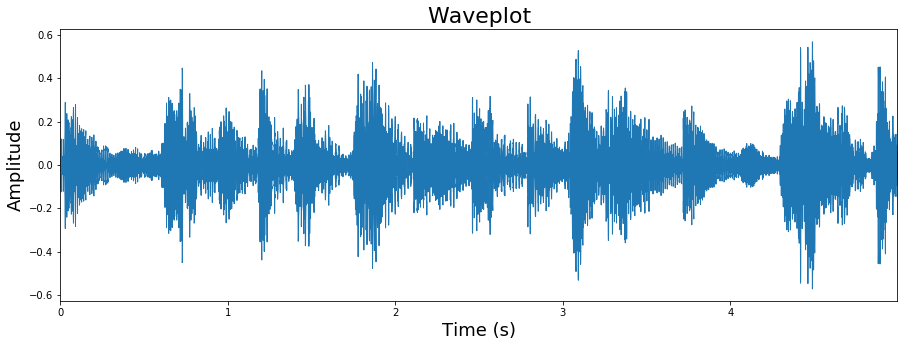
\includegraphics[scale=0.45]{img/Waveplot_Visualisation.png}
	\caption[Time-domain illustrated in wave plot]{Time-domain illustrated in wave plot}
	\label{fig:Waveplot-Time-Domain}
\end{figure}

\subsection{Frequency domain}
\label{sub:Frequency-Domain}
The frequency-domain refers to the analysis of mathematical functions or signals with respect to frequency. A frequency-domain graph shows how much of the signal lies within each given frequency band over a range of frequencies. 
\newline
\newline
A given function or signal can be converted between the time and the frequency domains with a pair of mathematical operators. The most used operation is the Fourier Transformation, which will be explained in further detail in section \ref{sub:Fourier-Transform}.

\subsection{Fourier transform}
\label{sub:Fourier-Transform}
\Gls{FT} is a mathematical concept that can convert a continuous signal from the time domain (\ref{sub:Time-Domain}) to frequency domain (\ref{sub:Frequency-Domain}). It decomposes a complex periodic signal into its constituent sine waves oscillating at different frequencies, along with the magnitude of each wave. The magnitude of each frequency shows how much a certain wave contributes to the overall signal.

\subsubsection{Fast Fourier transform}
\label{subsub:Fast-Fourier-Transform}
\Gls{FFT} is a mathematical algorithm that calculates \gls{DFT} of a given sequence, with equation \ref{eq:DFT}. The only difference between \gls{FT} and \gls{FFT} is that \gls{FT} considers a continuous signal while \gls{FFT} takes a discrete signal as input. \Gls{DFT} converts a sequence, a discrete signal, into its frequency constituents just like \gls{FT} does for a continuous signal. More precisely it is a transformation, which decomposes the signal into its base frequency building blocks. It is important to note that due to that transformation, the time information of the audio signal will be lost.

\myequations{Discrete Fourier Transform}
\begin{equation}
    \centering
    X_k = \sum_{n=0}^{N-1} \ x[n] \cdot e^{-\frac{i2\pi}{N}kn}
    \label{eq:DFT}
\end{equation}

\subsubsection{Short time Fourier transform}
\label{subsub:Short-Time-Fourier-Transform}
\Gls{STFT} is a mathematical algorithm which addresses the issue, that in the frequency domain (\ref{sub:Frequency-Domain}) no time information exists. The \gls{STFT} calculates several \gls{FFT} at different time intervals and combines them to get information about the signal varying over time.

\subsection{Spectrogram}
\label{sub:Spectrogram}
A spectrogram is a visual representation of the \gls{STFT} (\ref{subsub:Short-Time-Fourier-Transform}). More precisely it represents the spectrum of frequencies of a signal as it varies with time. The x-axis represents the time, the y-axis represents the frequencies, and the colours represent the magnitude of the observed frequency at a particular time. Bright colours represent powerful frequencies. Thus every spectrogram represents three domains: time, frequency and magnitude.
\newline
\newline
To create a spectrogram, the audio signal is broken down into smaller frames (windows), and for each one, the \gls{DFT} or \gls{FFT} will be calculated. The resulting frequencies of each window will represent the time. It is important to note that the windows should overlap each other, not to lose any frequency. Typical window sizes are 20 to 30ms, but this size highly depends on the task to solve. Figure \ref{fig:Spectrogram} shows an example of such a spectrogram.
\begin{figure}[htbp]
	\centering
	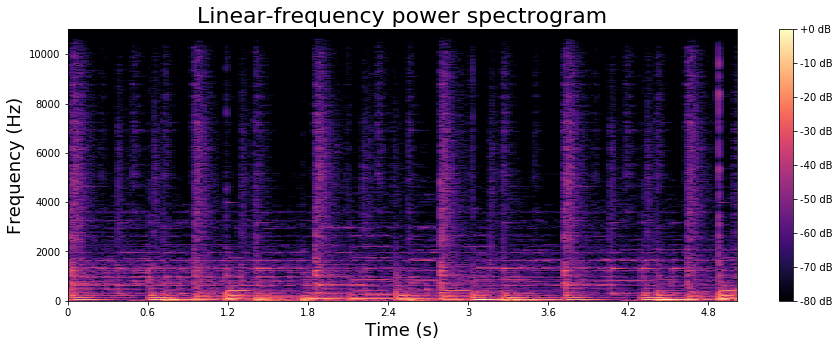
\includegraphics[scale=0.5]{img/Spectrogram_Visualisation.png}
	\caption[Example of a spectrogram]{Example of a spectrogram}
	\label{fig:Spectrogram}
\end{figure}

\subsection{Mel spectrogram}
\label{sub:Mel-Spectrogram}
\Glspl{MFCC} are a feature widely used in automatic speech and speaker recognition, mainly because they focus on the audio signal and discard all other information such as background noise, emotion and many more. They were introduced by Davis and Mermelstein in the 1980s, and have been state-of-the-art ever since.
\newline
\newline
The process of creating these \glspl{MFCC} are quite complex and follow five steps. Thus to the explanation of every step, there is also a short example on how to perform the step in depth. For illustration, a speech signal with a sample rate of 16kHz is assumed. The whole process is illustrated in figure \ref{fig:MFCC-Overview}.

\begin{figure}[htbp]
	\centering
    \begin{tikzpicture}[
        input/.style = {coordinate},
        output/.style = {coordinate},
        block/.style={rectangle, draw, text width=7.3em,
               text centered, rounded corners, minimum height=3em},
        arrow/.style={-{Stealth[]}}
    ]
        \node [input] (input) {};
        \node [block,right=3cm of input] (Frames)  {Break signal into overlapping frames};
        \node [block,right=of Frames] (FFT)  {Fast Fourier Transform (FFT)};
        \node [block,below right=0.2cm and 0.5cm of FFT] (MEL)  {Mel-Scale filter bank};
        \node [block,below left=0.2cm and 0.5cm of MEL] (LOG) {Log $|\cdot|$};
        \node [block,left=of LOG] (DCT) {Discrete Cosine Transform (DCT)};
        \node [output, left=3cm of DCT] (output) {};
    
        % Draw edges
        \draw [arrow] (input) -- (Frames) node [above,pos=0.25] {continuous audio} node [below,pos=0.25] {signal};
        \draw [arrow] (Frames) -- (FFT);
        \draw [arrow] (FFT)  -|  (MEL);  
        \draw [arrow] (MEL.south) |-  (LOG.east);  
        \draw [arrow] (LOG) -- (DCT) ;
        \draw [arrow] (DCT) -- node [above] {MFCC} (output);
    \end{tikzpicture}
    \caption{Steps to calculate MFCC}
    \label{fig:MFCC-Overview}
\end{figure}

\subsubsection{Frame the signal into short frames}
An audio signal is continuously changing, so to simplify it is assumed, that on short time scales the audio signal does not change much, i.e. statistically stationary. Due to that, the signal is framed into 20-40ms frames. If the frames are much shorter, there are not enough samples to get a reliable spectral estimate. If the frame length is too high, the signal changes to much throughout the frame.
\newline 
\newline
As a first step the signal has to be split into 20-40ms frames (normally 25ms is standard). The frame length for a 16kHz signal is calculated with the equation in \ref{eq:MFCC-Frame-Length}. 
\myequations{Calculate frame length from signal}
\begin{equation}
    \centering
    0.025s * 16000Hz = 400 \ \text{samples}
    \label{eq:MFCC-Frame-Length}
\end{equation}
Frame step is normally 10ms, which allows some overlap to the frames, and is calculated the same as the frame length.
\myequations{Calculate frame step from signal}
\begin{equation}
    \centering
    0.01s * 16000Hz = 160 \ \text{samples}
    \label{eq:MFCC-Frame-Step}
\end{equation}
This means that the first 400 samples start at 0, the next 400 frames start at sample 160, until the end of the speech signal is reached. If the speech signal does not divide into an even number of frames, it is padded with zeros until it does. The next steps within the example are applied to every single frame. Thus for every frame a set of features will be extracted, in this case a set of \glspl{MFCC}.

\subsubsection{Calculate the periodogram estimate of the power spectrum for each frame}
The next step is to calculate the power spectrum of each frame. This is motivated by the human cochlea, an organ in the ear, which vibrates at different spots depending on the frequency of the incoming sounds. Depending on which location in the cochlea vibrates, different nerve fibre fire, informing the brain that specific frequencies are present. The periodogram estimate performs a similar job which is, identifying which frequencies are present in the frame.
\newline
\newline
To calculate the power spectrum for each frame, the \gls{DFT} has to be calculated with equation \ref{eq:MFCC-DFT-Frame}. Then the Periodogram-based power spectral estimate for the speech frame $s_i[n]$ can be calculated with the formula \ref{eq:MFCC-Periodogram-Frame}. Usually, a 512 point \gls{DFT} is being performed, which decomposes the signal frame $s_i[n]$ into 512 frequency building blocks and only the first 257 coefficients are kept.
\myequations{Calculate Discrete Fourier Transform of each frame}
\begin{equation}
    \centering
    S_i[k] = \sum_{n=1}^{N} s_i[n] \ h[n] \ e^{- \frac{i2\pi}{N} kn} \qquad 1 \leq k \leq K
    \label{eq:MFCC-DFT-Frame}
\end{equation}
\myequations{Calculate Periodogram-based power spectral estimate of each frame}
\begin{equation}
    \centering
    P_i[k] = \frac{1}{N}\Big|S_i[k]\Big|^2
    \label{eq:MFCC-Periodogram-Frame}
\end{equation}
where:
\begin{conditions*}
 s_i[n] &  time-domain signal frame, where $N$ denotes the frame length (in the current example from 1-400), and $i$ ranges over the number of frames \\   
 S_i[k] &  complex \gls{DFT}, where $i$ denotes the frame number corresponding to the time-domain frame \\
 h[n]   &  analysis window, with the size $N$ (e.g. hamming window) \\
 K      &  length of the \gls{DFT} \\
 P_i[k] &  power spectrum of frame $i$
\end{conditions*}

\subsubsection{Apply the Mel filterbank to the power spectra}
The periodogram spectral estimate still contains a lot of information, which does not provide any performance gain and can therefore be further compressed. In the human body, the cochlea can not discern the difference between two closely spaced frequencies. This effect becomes more pronounced as the frequencies increase. For this reason, clumps of periodogram bins and sums are taken and summed up, to get an idea of how much energy exists in various frequency regions.
\newline
\newline
The Mel filterbank performs this step. The first filter of the filterbank is very narrow and indicates how much energy exists near 0 Hertz. As the frequencies get higher, the filters get wider as the variations become less relevant. The interest is only focused on how much energy occurs at each spot. The Mel scale gives the spacing and the wideness of the filterbanks. It relates perceived frequency, or pitch, of a pure tone to its actual measured frequency, it transforms the features to match more closely what humans hear. The equation \ref{eq:MFCC-Mel} converts a frequency ($f$) to the Mel scale ($m$) and equation \ref{eq:MFCC-Mel-Inv} transforms the Mels ($m$) back to a frequency ($f$).\footnote{\fullcite{anne_acoustic_2015}}
\myequations{Calculate Mel scale from frequency}
\begin{equation}
    \centering
    m = 2595 \ log_{10}(1 + \frac{f}{700Hz}) = 1127 \ log_e(1 + \frac{f}{700Hz})
    \label{eq:MFCC-Mel}
\end{equation}
\myequations{Calculate frequency from Mel scale}
\begin{equation}
    \centering
    f = 700 \ (10^{m/2595-1}) = 700 \ (e^{m/1127-1})
    \label{eq:MFCC-Mel-Inv}
\end{equation}
The Mel-spaced filterbank has to be computed to apply the filterbank to the power spectra. The filterbank is a set of 20-40 (26 is the standard) triangular filters that then are applied to the periodogram from before. The filterbank has the dimension of 26 vectors with the length 257, because in the step before the \gls{FFT} was calculated and only kept 257 coefficients. Each vector has mostly zeros in it but is non-zero for a specific section of the spectrum. Each filterbank has to be multiplied by the power spectrum. After that, the coefficients are added up to get the filterbank energies. In the end, there are 26 coefficients left, which indicates how much energy was in each filterbank. An example of a Mel-spaced filterbank is illustrated in \ref{fig:MFCC-Mel-Filterbank}.
\begin{figure}[htbp]
	\centering
	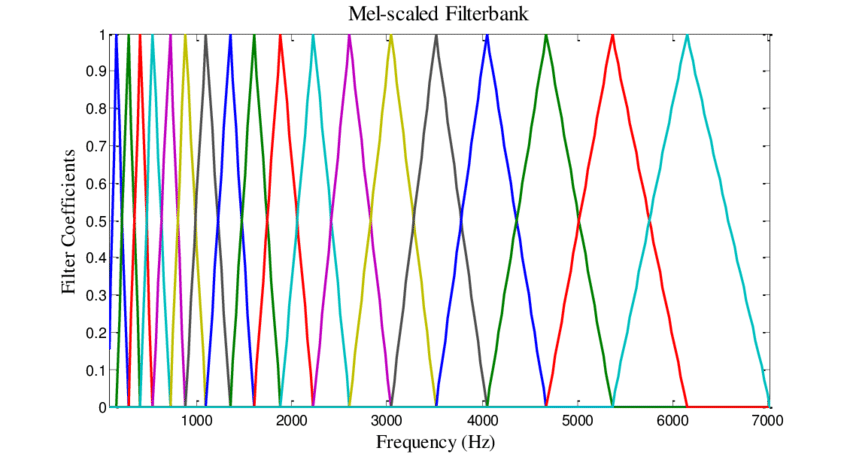
\includegraphics[scale=0.4]{img/Mel-filter-banks-basis-functions-using-20-Mel-filters-in-the-filter-bank.png}
	\caption[Mel-spaced filterbank with 20 filters]{Mel-spaced filterbank with 20 filters \footnotemark}
	\label{fig:MFCC-Mel-Filterbank}
\end{figure}
\footnotetext{\fullcite{mohd_ali_analysis_2013}}

\subsubsection{Apply the logarithm to all filterbank energies}
After the calculation of the filterbank energies, the logarithm is applied to each one of them. This operation is also inspired by human hearing because humans do not hear loudness on a linear scale. Generally to double the perceived volume of a sound eight times as much energy has to be put in. Thus if the sound signal is loud in the beginning, significant variations in energy may not sound that different. The output of this step can be visualised in a log-mel spectrogram, which is also an essential feature in audio processing.
\newline
\newline
In the above example, there are 26 energy coefficients which will be logarithmized and leaves 26 log filterbank energies.

\subsubsection{Apply the \gls{DCT} to the log filterbank energies}
The final step is to compute the \gls{DCT} of the log filterbank energies. Mainly because the filterbanks are all overlapping and are correlated with each other. The \gls{DCT} decorrelates the energies, but only the lower 12-13 of the 26 \gls{DCT} coefficients are kept. This is because the higher \gls{DCT} coefficients represent fast changes in the filterbank energies, and these fast changes can degrade the \gls{ASR} performance.
\newline
\newline
In the example, the \gls{DCT} of the 26 log filterbank energies has to be computed, which gives 26 cepstral coefficients. This whole process has to be calculated for each frame in the signal.

\subsubsection{Visualize the cepstral coefficients}
Once all the cepstral coefficients are computed, they can be visualized with respect to time. Which then can be used for further processing in \gls{ASR}. Such a visualisation is illustrated in figure \ref{fig:MFCC-Visualisation}, where the x-axis represents the time, and the y-axis represents the cepstral coefficient dimension (e.g. the lower 12-13), and the colour shows the value of each coefficient.
\begin{figure}[htbp]
	\centering
	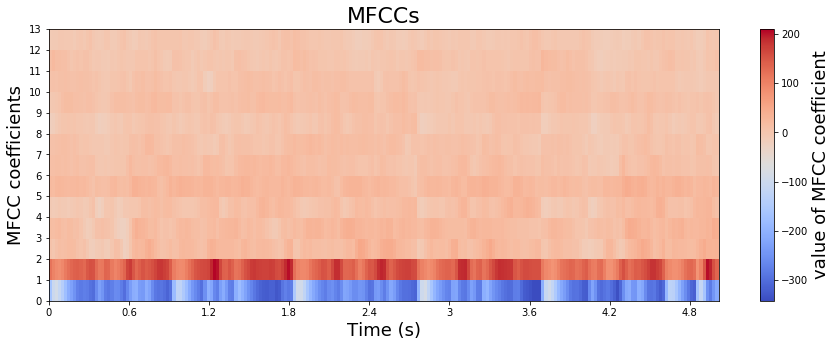
\includegraphics[scale=0.5]{img/MFCC_Visualisation.png}
	\caption[Visualisation of an MFCC]{Visualisation of a MFCC}
	\label{fig:MFCC-Visualisation}
\end{figure}

\subsection{LibROSA}
\label{sub:Librosa}
LibROSA is a python package for audio analysis and processing. At a high level, libROSA provides implementations of a variety of standard functions used throughout the field of music information retrieval. Because of this variety of realised functions, it quickly became the state-of-the-art in the field of machine learning for audio. It can easily be installed on any machine using PIP.\footnote{\url{https://librosa.github.io/librosa/}}

\begin{verbatim}
    pip install librosa
\end{verbatim}

\section{Introduction to neural networks}
\label{sec:Intro-NN}
This section provides an introduction to an essential concept in this thesis, neural networks. They will be used to build the model and tackle the problem. First, a general neural network (\ref{sub:Neural-Network}) is introduced to clarify some terminology. After that, convolutional neural network (\ref{sub:Convolutional-Neural-Network}) and gated recurrent unit (\ref{sub:Gated-Recurrent-Unit}) will be explained to give an overview of some specialized kind of neural networks.

\subsection{Neural network}
\label{sub:Neural-Network}

\begin{figure}[htbp]
    \centering
    \begin{tikzpicture}
    
    \def\nodedist{45pt}
    \def\layerdist{70pt}
    \def\pindist{20pt}
    
    \tikzstyle{every pin edge}=[signal]
    \tikzstyle{annot} = [text width=4em, text centered]
    
    % input nodes
    \foreach \y in {1,...,3}
        \node[inputnode, pin={[pin edge={latex-}, pin distance=\pindist]left:Input \y}] 
            (x\y) at (0,-\y*\nodedist) {$x_\y$};
    
    % sum
    \node[infonode] 
            (sigma) at ($(x2) + (\layerdist, -0*\nodedist)$) {$\displaystyle\Sigma$};
            
    % bias
    \node[inputnode, label=above:{\parbox{2cm}{\centering Bias}}] at (sigma|-x1) (b1) {$b_1$};
    
    % activation function
    \node[infonode, label=above:{\parbox{2cm}{\centering Activation\\ function}}] 
            (activation) at ($(sigma) + (\layerdist, -0*\nodedist)$) {$f(z)$};
            
    % output node
    \node[outputnode, pin={[pin edge={-latex}, pin distance=\pindist]right:Output}]
            (output) at ($(activation) + (\layerdist, -0*\nodedist)$) {$\hat{y}$};
    
    % arrows 
    \draw[signal] (x1) -- (sigma) node [below right=0.25 and 0.05 of x1] {$\theta_{1}$};
    \draw[signal] (x2) -- (sigma) node [below right=-0.1 and 0.05 of x2] {$\theta_{2}$};
    \draw[signal] (x3) -- (sigma) node [below right=-0.5 and 0.05 of x3] {$\theta_{3}$};
    \draw[signal] (b1) -- (sigma);
    \draw[signal] (sigma) -- (activation);
    \draw[signal] (activation) -- (output);
    
    \end{tikzpicture}
    \caption{Visualization of a perceptron}
    \label{fig:Perceptron-Visualisation}
\end{figure}
\noindent
Warren McCulloch and Walter Pitts introduced the first \gls{NN} in 1943 within the paper (\cite{mcculloch_logical_1943}), where they proposed a computational model for a \gls{NN} based on algorithms called threshold logic. To develop the \gls{NN}, they used observations about the neurophysiology of the brain. In simplified terms, the brain can be described similar to a net of neurons where each neuron has a soma and an axon. The soma denotes the corpus of the neuron and the axon a nerve’s extension for the connection with others. Synapses exist between the axon of one neuron and the soma of another. The neuron sends an impulse if its excitation exceeds a certain threshold. Later in 1958 Frank Rosenblatt extended this idea of a \gls{NN} to the Perceptron formulation (\cite{rosenblatt_perceptron_1958}). It is one of many neuron representations which have been used within neural networks so far.
\newline
\newline
A perceptron is the simplest neural network which consists of $n$ number of inputs and only one output. It further consists of multiple inputs, multiple weights, a bias, an activation function and an output. The building blocks and the procedure of calculating an output are visualised in figure \ref{fig:Perceptron-Visualisation}.

\begin{figure}[htbp]
    \centering
    \subfloat[Sigmoid]{
            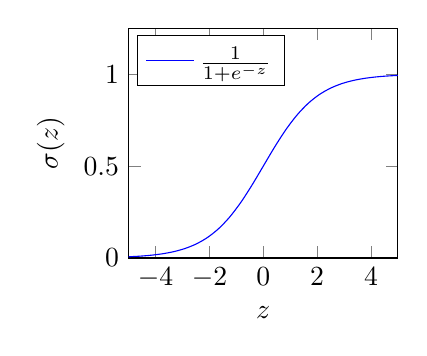
\begin{tikzpicture}
            \begin{axis}[legend pos=north west, width=5cm,height=4.5cm,ylabel=$\sigma(z)$,xlabel=$z$,ymin=0,ymax=1.25,xmin=-5,xmax=5]
                \addplot[blue,smooth] {1/(1+exp(-x))};
                \addlegendentry{$\frac{1}{1+e^{-z}}$}
            \end{axis}
        \end{tikzpicture}
    }
    \subfloat[Tanh]{
        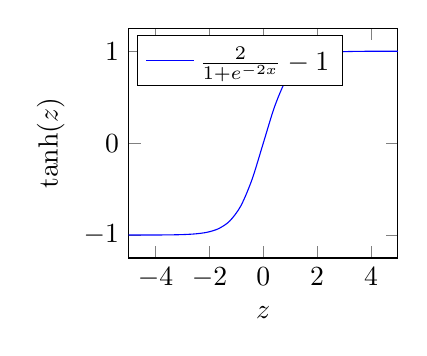
\begin{tikzpicture}
            \begin{axis}[legend pos=north west, width=5cm,height=4.5cm,ylabel=$\tanh(z)$,xlabel=$z$,ymin=-1.25,ymax=1.25,xmin=-5,xmax=5]
                \addplot[blue,smooth] {tanh(x)};
                \addlegendentry{$\frac{2}{1+e^{-2x}} -1$}
            \end{axis}
        \end{tikzpicture}
    }
    \subfloat[ReLU]{
            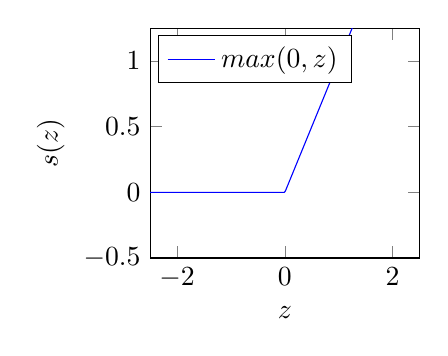
\begin{tikzpicture}
            \begin{axis}[legend pos=north west, width=5cm,height=4.5cm,ylabel=$s(z)$,xlabel=$z$,ymin=-0.5,ymax=1.25,xmin=-2.5,xmax=2.5]
                \addplot[samples=500, blue] {max(0, x)};
                \addlegendentry{$max(0, z)$}
            \end{axis}
        \end{tikzpicture}
    }
    \caption{Graphical representation of non-linear activation functions}
    \label{fig:Activation-Functions}
\end{figure}
\noindent
The inputs which are denoted as $x_1, \dots, x_n$, are the values passed into the perceptron. The weights $\theta_{1}, \dots, \theta_{n}$ are values which are multiplied with the respective input, the bias is a special weight which shifts the activation function to the left or right. And the activation function $f(z)$ is used to introduce non-linearity into the output. Without the \gls{NN} would represent a linear function. With the non-linearity of the activation function, a layered \gls{NN} with enough capacity can learn any function. Such non-linear activation functions are illustrated in figure \ref{fig:Activation-Functions}. The output $\hat{y}$ is simply the result of the activation function, and it can be computed using equation \ref{eq:Perceptron-Calculate-Output}. In the case of a perceptron, it is the output of the \gls{NN}. The process of calculating the output of a \gls{NN} is called forward propagation.
\myequations{Calculates the output of single layer neural network}
\begin{equation}
    \centering
    \hat{y} = f(z) = f\Big(b_1 + \sum_{i=1}^n x_i \theta_i \Big)
    \label{eq:Perceptron-Calculate-Output}
\end{equation}
In deeper networks, the output of one layer is then used again as the input of the next layer $f^L(f^{L-1}(\cdots f^1(z)))$, where $L$ denotes the number of layers in the \gls{NN}. A layer consists of multiple perceptrons. Thus this is often called a \gls{MLP}, which is illustrated in figure \ref{fig:MLP-Visualisation}. $z_1^1$ is one example of a single perceptron within the network. The \gls{MLP} shown in figure \ref{fig:MLP-Visualisation} has four layers ($L = 4$), from which the first one is always the input layer, and the last one is the output layer. The layers between the input and output layer are called hidden layers. These layers are also called fully connected layers, because there is a corresponding weight to each input of the next layer.

\begin{figure}[htbp]
    \centering
    \begin{tikzpicture}[]
        \def\nodedist{35pt}
        \def\layerdist{80pt}
        \def\pindist{20pt}
        
        \tikzstyle{every pin edge}=[signal]
        \tikzstyle{annot} = [text width=4em, text centered]
        
        \foreach \y in {1,...,3}
            \node[inputnode, pin={[pin edge={latex-}, pin distance=\pindist]left:Input \y}] 
                (I\y) at (0,-\y*\nodedist) {$x_\y$};  
    
        \foreach \y in {1,...,4}
            \node[hiddennode] 
                (H1\y) at ($(\layerdist,-\y*\nodedist) +(0, 0.5*\nodedist)$) {$z_\y^1$};
        
        \foreach \y in {1,...,4}
            \node[hiddennode] 
                (H2\y) at ($(2*\layerdist,-\y*\nodedist) +(0, 0.5*\nodedist)$) {$z_\y^2$};
        
        \foreach \y in {1,...,2}
            \node[outputnode, pin={[pin edge={-latex}, pin distance=\pindist]right:Output \y}]
                (O\y) at ($(H21) + (\layerdist, -\y*\nodedist)$) {$\hat{y}_\y$};
    
        \foreach \dest in {1,...,4}
            \foreach \source in {1,...,3}
                \draw[signal] (I\source) -- (H1\dest);
        
        \foreach \dest in {1,...,4}
            \foreach \source in {1,...,4}
                \draw[signal] (H1\source) -- (H2\dest);
        
        \foreach \dest in {1,...,2}
            \foreach \source in {1,...,4}
                \draw[signal] (H2\source) edge (O\dest);
    
        \node[annot, above=4pt of H11] (hl) {Hidden layer 1};
        \node[annot, above=4pt of H21] (hl) {Hidden layer 2};
        \node[annot] at (I1 |- hl) {Input layer};
        \node[annot] at (O1 |- hl) {Output layer};
    \end{tikzpicture}
    \caption{Visualization of a multilevel perceptron}
    \label{fig:MLP-Visualisation}
\end{figure}
\noindent
In order that the \gls{NN} produces more reliable results, it has to learn the optimal parameters for a given problem. This procedure consists of two parts, backpropagation and optimisation. Backpropagation refers to the algorithm for computing the gradient of the loss function with respect to the parameters, to see how good the current predictions are. However, the term is often used to refer to the entire learning algorithm, including optimization. Furthermore, optimisation is the process of selecting the best element from some set of available alternatives, which in the case of a \gls{NN} is the selection of the best parameters.
\newline
\newline
The first step in backpropagation is to know an estimation of how far away the current predictions are from the desired solution, which can be computed using a loss function. Typical loss functions are \gls{MSE}, binary cross-entropy, categorical cross-entropy or sparse categorical cross-entropy. The process of selecting the right loss function highly depends on the problem to solve. The equation \ref{eq:MSE} defines the \gls{MSE} cost (loss) function $\mathcal{L}$ for the entire dataset with size $n$.
\myequations{Mean Squared Error loss function for entire dataset}
\begin{equation}
    \centering
    \mathcal{L} = MSE = \frac{1}{n} \sum_{i=1}^n(y_i - \hat{y}_i)^2
    \label{eq:MSE}
\end{equation}
where:
\begin{conditions*}
    y_i & actual value from the dataset \\   
    \hat{y}_i & predicted value, output of the \gls{NN}
\end{conditions*}
\noindent
The next step in backpropagation is to calculate the error of each weight $\theta_i$. The bias $b_i$ can also be thought of as a special kind of weight within the network. This is done by computing the gradients, given the cost function $\mathcal{L}$, with respect to the weights $\theta_i$. The gradient can be interpreted as the direction and rate of fastest increase. 
\newline
\newline
In equation \ref{eq:Backpropagation-Gradient} the gradient of the cost function $\mathcal{L}$ with respect to the weights $\theta_i$ is computed using partial derivation. The equation computes the gradients of the weights from the last hidden layer (\flqq Hidden layer 2\frqq, e.g. $z^2_1$) shown in figure \ref{fig:MLP-Visualisation}. For lower layers, the chain rule would be used more extensively. The same function can also be used to compute the cost function $\mathcal{L}$ with respect to the bias. Since the cost function is not directly related to the weights, the chain rule is used.
\myequations{Gradient of cost function with respect to the weights}
\begin{equation}
    \centering
    \frac{\partial \mathcal{L}}{\partial\theta_i} = \frac{\partial \mathcal{L}}{\partial\hat{y}}\times\frac{\partial\hat{y}}{\partial z}\times\frac{\partial z}{\partial\theta_i}
    \label{eq:Backpropagation-Gradient}
\end{equation}
The last step in the learning process of a \gls{NN} is the optimisation. Gradient descent is one of many optimisation algorithms, and it changes the weights and bias, proportional to the negative of the gradient of the cost function with respect to the corresponding weight or bias. Learning rate $\alpha$ is a hyperparameter, which is used to control how much the weights and bias change. The weights and bias are updated with equations \ref{eq:Optimisation-Gradient-Descent-Weights}.
\myequations{Optimisation of weights using gradient descent}
\begin{equation}
    \centering
    \theta_i = \theta_i - \Big(\alpha \times \frac{\partial \mathcal{L}}{\partial\theta_i}\Big)
    \label{eq:Optimisation-Gradient-Descent-Weights}
\end{equation}
The whole learning process consisting of backpropagation and optimisation is repeated until the \gls{NN} convergences in a local or global minimum.
\newline
\newline
\gls{MLP} have several drawbacks, especially when it comes to handling two-dimensional data, for example, audio or image data. \gls{MLP} use one perceptron for each input (e.g. pixel in an image, multiplied by 3 in the case of RGB). The amount of weights rapidly becomes unmanageable for large input data. In case of a 224 x 224 pixel image with three colour channels, there are around 150'000 weights that must be trained. As a result, difficulties arise while training and overfitting can occur. Another common problem is that \gls{MLP} react differently to an input and its shifted version — they are not translation invariant. For example, if a picture of a cat shows the cat is located in the top left corner of one of the images, the \gls{MLP} will try to update the weights accordingly and assume that all of the cats will appear in this section of the image. All the problems stated above also apply to other areas. Thus \gls{MLP} are not ideal for processing two-dimensional data. In the next section, convolutional neural network (\ref{sub:Convolutional-Neural-Network}) will be introduced, which will solve the problems stated above.

\subsection{Convolutional neural network}
\label{sub:Convolutional-Neural-Network}
\Gls{CNN} is a specific kind of neural network for processing data that has a known grid-like topology. Examples include time-series data, which can be thought of as a 1-D grid taking samples at regular time intervals, and image data, which can be thought of as a 2-D grid of pixels. The name \flqq convolutional neural network\frqq \ indicates that the network employs a mathematical operation called convolution. Convolution is a specialized kind of linear operation. To summarize, \glspl{CNN} are neural networks that use the convolution operation instead of general matrix multiplication in at least one of their layers. \footnote{\fullcite{goodfellow_deep_2016}}
\newline
\newline
A typical layer of a \gls{CNN} consists of three stages, which is illustrated in figure \ref{fig:Convolution-Layer-Visualisation}. In the first stage, the layer performs several convolutions in parallel to produce a set of linear activations, also called a feature map. In the second stage, each linear activation is run through a non-linear activation function, such as the rectified linear activation function. This stage is sometimes called the detector stage. In the third stage, a pooling function is used to modify the output of the layer further.

\begin{figure}[htbp]
    \captionsetup{format=plain}
    \centering
    \begin{tikzpicture}[start chain=going below, node distance=15pt,
        point/.append style={on chain, join=by {signal}},
        layer/.append style={on chain, join=by {signal}},
    ]
        \node[point] {Input to layers};
        \node[conv] {Convolution layer: \\ affine transform};
        \node[activation] {Detector layer: \\ non-linearity (e.g., ReLU)};
        \node[pool] {Pooling layer};
        \node[point] {Next layer};
    \end{tikzpicture}
    \caption{Visualisation of a single convolutional layer}
    \label{fig:Convolution-Layer-Visualisation}
\end{figure}
\noindent
Convolution is a process where a small matrix of numbers, called the kernel or filter, is taken and slid it over grid-like data (e.g. an image) and transforms it based on the values from the filter. More concretely, at a given position of the convolution kernel, the element-wise multiplication of each kernel cell value and the corresponding image pixel value that overlaps the kernel cell is taken and then summed up. The convolutional operation is often denoted as $\ast$, the equation \ref{eq:Convolution} shows how to calculate the convolution of an input image $I$ and a two-dimensional filter kernel $K$ with the filter size $(m, n)$. The rows and the columns of the input image $I$ are denoted as $i$ and $j$. The output of the convolutional operation $S(i,j)$ is often called the feature map. A visualisation of the operation is illustrated in figure \ref{fig:Convolution-Visualisation}. In the context of \glspl{CNN}, the learning algorithm will learn the appropriate values of the kernel in the appropriate place, to detect arbitrary features.
\myequations{Convolution of an image and a two-dimensional kernel}
\begin{equation}
    \centering
    S(i,j) = (K \ast I)(i,j) = \sum_{m=-\infty}^\infty \sum_{n=-\infty}^\infty I(i-m, j-n) \cdot K(m,n)
    \label{eq:Convolution}
\end{equation}
The goal of the convolutional operation within the \gls{CNN} is to output a high value for a given position, if the kernel is present in that location, otherwise it outputs a low value. The convolutions are restricted to only \flqq valid\frqq \ positions, where the kernel lies entirely within the image. Since the image shrinks every time a convolution is performed, it can only be performed a limited number of times. Furthermore, it can be seen that the kernel has a more significant impact on the centre of the image than on the outskirts. The image will be padded with an additional border, to solve both of these problems. Usually, it is filled with zeros. Depending on whether padding is used or not, there are two types of convolution: Valid and Same. Valid means that the original image is used and same states, that padding around the image is used and thus the input and output image have the same size. Another important hyperparameter of a \gls{CNN} is stride, which indicates how much the kernel slides to its next position. Figure \ref{fig:Convolution-Visualisation} illustrates a convolution with a 2x2 kernel, padding valid and stride one. 

\begin{figure}[htbp]
    \captionsetup{format=plain}
    \centering
    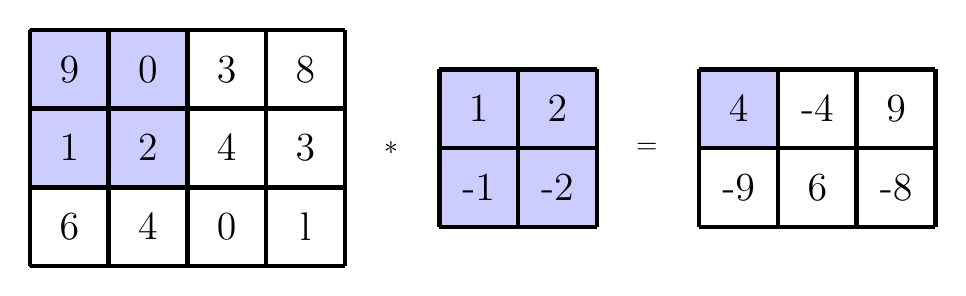
\begin{tikzpicture}
        \coordinate (p) at (0,0);
        \draw[shift={(p)}, fill=white] (0,0) rectangle (4,-3);
        \draw[shift={(p)}, fill=blue!20!white] (0,0) rectangle (2,-2);
        \draw[
            ultra thick,
            step=1, 
            color=black,
            draw=black,
            fill=black!20!white,
            shift={(p)}
        ] (0,0) grid (4,-3)
        foreach[count=~] \l in {9, 0, 3, 8, 1, 2, 4, 3, 6, 4, 0, l} {
            ({0.5+mod(~-1,4}, {-0.5-div(~-1,4}) node {\Large \l}
        };
        
        \node[text width=1cm] at (5,-1.5) {$\Large\ast$};
        
        \coordinate (p) at (5.2,-0.5);
        \draw[shift={(p)}, fill=blue!20!white] (0,0) rectangle (2,-2);
        \draw[
            ultra thick,
            step=1, 
            color=black,
            draw=black,
            fill=black!20!white,
            shift={(p)}
        ] (0,0) grid (2,-2)
        foreach[count=~] \l in {1, 2, -1, -2} {
            ({0.5+mod(~-1,2}, {-0.5-div(~-1,2}) node {\Large \l}
        };
        
        \node[text width=1cm] at (8.2,-1.5) {$\Large =$};
        
        \coordinate (p) at (8.5,-0.5);
        \draw[shift={(p)}, fill=white] (0,0) rectangle (3,-2);
        \draw[shift={(p)}, fill=blue!20!white] (0,0) rectangle (1,-1);
        \draw[
            ultra thick,
            step=1, 
            color=black,
            draw=black,
            fill=black!20!white,
            shift={(p)}
        ] (0,0) grid (3,-2)
        foreach[count=~] \l in {4, -4, 9, -9, 6, -8} {
            ({0.5+mod(~-1,3}, {-0.5-div(~-1,3}) node {\Large \l}
        };
    \end{tikzpicture}
    \caption[Visualization of a convolutional operation]{Visualization of a convolutional operation. To calculate the value highlighted in blue within the feature map (right), the equation \ref{eq:Convolution} has to be used. Thus the highlighted element can be calculated with $9\cdot 1 + 0\cdot 2 + 1\cdot (-1) + 2\cdot (-2) = 4$}
    \label{fig:Convolution-Visualisation}
\end{figure}
\noindent
A pooling function replaces the output of the net at a particular location with a summary statistic of the nearby outputs. For example, the max-pooling operation reports the maximum output within a rectangular neighbourhood. Another popular pooling function is the average-pooling, which outputs the average number within a rectangular neighbourhood. Both pooling functions are illustrated in figure \ref{fig:Pooling-Visualisation}. Pooling helps to make the representation approximately invariant to small translations of the input. Invariance to translation means that if a small amount translates the input data, the values of most of the pooled outputs do not change. Invariance to local translation can be a useful property if the focus is more on whether some feature is present within the data than exactly where it is located.

\begin{figure}[htbp]
    \centering
    \begin{tikzpicture}
        \coordinate (p) at (0,0);
        \draw[shift={(p)}, fill=red!20!white] (0,0) rectangle (2,-2);
        \draw[shift={(p)}, fill=yellow!20!white] (2,0) rectangle (4,-2);
        \draw[shift={(p)}, fill=blue!20!white] (0,-2) rectangle (2,-4);
        \draw[shift={(p)}, fill=green!20!white] (2,-2) rectangle (4,-4);
        \draw[
            ultra thick,
            step=1, 
            color=black,
            draw=black,
            fill=black!20!white,
            shift={(p)}
        ] (0,0) grid (4,-4)
        foreach[count=~] \l in {73, 74, 17, 49, 10, 29, 41, 20, 4, 23, 39, 4, 50, 80, 56, 57} {
            ({0.5+mod(~-1,4}, {-0.5-div(~-1,4}) node {\Large \l}
        };
        
        % max pooling
        \coordinate (p) at (7,0.5);
        \draw[shift={(p)}, fill=red!20!white] (0,0) rectangle (1,-1);
        \draw[shift={(p)}, fill=yellow!20!white] (1,0) rectangle (2,-1);
        \draw[shift={(p)}, fill=blue!20!white] (0,-1) rectangle (1,-2);
        \draw[shift={(p)}, fill=green!20!white] (1,-1) rectangle (2,-2);
        \draw[
            ultra thick,
            step=1, 
            color=black,
            draw=black,
            fill=black!20!white,
            shift={(p)}
        ] (0,0) grid (2,-2)
        foreach[count=~] \l in {74, 49, 80, 57} {
            ({0.5+mod(~-1,2}, {-0.5-div(~-1,2}) node {\Large \l}
        };
        \draw[signal] (4.5,-1.5) -> ($(p) +(-0.5, -1.25)$);
        \node[text width=100pt, align=center, right of=p, yshift=10pt] (l1) {Max-Pooling};
        
        % average pooling
        \coordinate (p) at (7,-2.5);
        \draw[shift={(p)}, fill=red!20!white] (0,0) rectangle (1,-1);
        \draw[shift={(p)}, fill=yellow!20!white] (1,0) rectangle (2,-1);
        \draw[shift={(p)}, fill=blue!20!white] (0,-1) rectangle (1,-2);
        \draw[shift={(p)}, fill=green!20!white] (1,-1) rectangle (2,-2);
        \draw[
            ultra thick,
            step=1, 
            color=black,
            draw=black,
            fill=black!20!white,
            shift={(p)}
        ] (0,0) grid (2,-2)
        foreach[count=~] \l in {46, 32, 39, 39} {
            ({0.5+mod(~-1,2}, {-0.5-div(~-1,2}) node {\Large \l}
        };
        \draw[signal] (4.5,-2.5) -> ($(p) +(-0.5, -0.75)$);
        \node[text width=100pt, align=center, right of=p, yshift=10pt] (l1) {Average-Pooling};
    \end{tikzpicture}
    \caption{Visualisation of the max- and average-pooling operation}
    \label{fig:Pooling-Visualisation}
\end{figure}
\noindent
Almost every \gls{CNN} has some fully connected layers in the last layer because they will combine the features learnt by different convolution kernels so that the network can build a global representation about the holistic input data. The neurons in the fully connected layer will get activated based on whether various entries, represented by convolution features, are present in the inputs. This provides a compact representation of features existing in the input to the output layer, which the output layer can easily use to classify the input data correctly.
\newline
\newline
To create a \gls{CNN}, all of the above concepts have to be put together to form an end-to-end model, from a raw input data to a decision. To summarise, the convolution layers will learn various local features in the data (e.g. what an eye looks like), then the pooling layer will make the \gls{CNN} invariant to translations of these features (e.g. if the eye appears slightly translated in two images, the \gls{CNN} will still recognise it as an eye). Finally, the fully connected layers combine the found features and activate the correct output (e.g. there are two eyes, a nose and a mouth, this must be a person).

\subsubsection{Dilated convolution}
\label{subsub:Dilated-Convolution}
Dilated convolution is a specialized type of convolution, which was first introduced within the paper (\cite{yu_multi-scale_2016}). It is helpful first to understand why vanilla convolutions (normal convolutions) struggle to integrate the global context. Suppose a purely convolutional network composed of layers of $k \times k$ convolutions, without pooling. It is clear to see that size of the receptive field of each unit (the block of pixels which can influence its activation) is $l \times (k-1) + k$, where $l$ is the layer index. Therefore the effective receptive field of units can only grow-linearly with the layers. Especially for high-resolution input images, the linearly-grow is very limiting.
\newline
\newline
Dilated convolutions increase the kernel by inserting spaces between the kernel elements. The dilation rate is controlled by an additional hyperparameter $l$. These one dimensional dilated convolutions between signal $I$ and kernel $K$ and dilation factor $l$ is defined by formula \ref{eq:Dilated-Convolution}. $\ast_l$ refers to the dilated convolution or a $l$-dilated convolution. The normal convolution $\ast$ is simply the 1-dilated-convolution. The figure \ref{fig:Dilated-Convolution} illustrates stacked dilated convolutions within a \gls{CNN}, where the dilation factor $l$ is increased exponentially.
\myequations{Convolution of an image and a two-dimensional kernel}
\begin{equation}
    \centering
    (K \ast_l I)(i) = \sum_{n=-\infty}^\infty K(n) \cdot I(i - ln)
    \label{eq:Dilated-Convolution}
\end{equation}
Dilated convolutions are used to cheaply increase the receptive field of output units without increasing the kernel size, which is especially useful when multiple dilated convolutions are stacked one after another. For a concrete example, see \cite{oord_wavenet_2016}, in which the proposed WaveNet model implements an autoregressive generative model for raw audio which uses dilated convolutions to condition new audio frames on a broad context of past audio frames.

\begin{figure}[htbp]
	\centering
	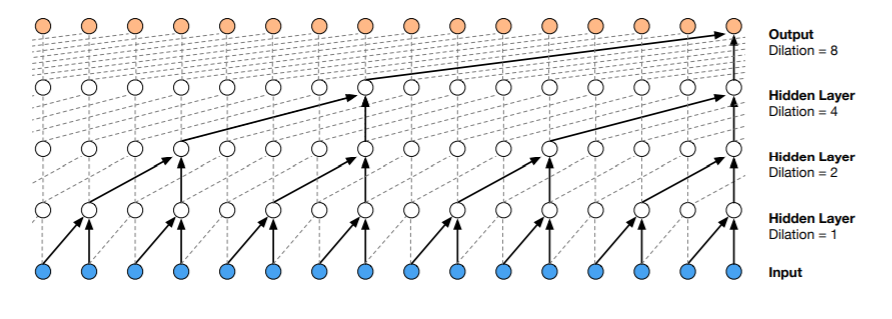
\includegraphics[scale=0.9]{img/Dilated_Colvolution.png}
	\caption[SINS database recording environment map]{Visualisation of stacked diluted convolutions \footnotemark}
	\label{fig:Dilated-Convolution}
\end{figure}
\footnotetext{\fullcite{oord_wavenet_2016}}

\subsection{Gated recurrent unit}
\label{sub:Gated-Recurrent-Unit}
\Gls{GRU} is a specialised type of \glspl{NN} within the family of \glspl{RNN}, which focus on processing sequential data. \glspl{GRU} were introduced in the paper (\cite{cho_learning_2014}) to solve the vanishing gradient problem, which comes with a standard \gls{RNN}. \gls{RNN} take as their input, not just the current input example they see, but also what they have perceived previously. It can be thought of multiple feed-forward neural networks, passing information from one to the other. The vanishing gradient problem states that input from far behind (e.g. the first sample in a sequence) loses its importance in the last inputs (e.g. the last sample of a sequence), because it vanishes along the way.

\begin{figure}[htbp]
    \captionsetup{format=plain}
    \centering
    \begin{tikzpicture}[thick, node distance=30pt and 30pt, on grid]
        \node[cell, minimum width=200pt, minimum height=110pt, anchor=north west] (b) at (-2pt,0pt) {};
        
        \coordinate (hin) at (0pt,-20pt);
        \draw[signal] (hin) +(-\iolen, 0pt) node[above] {$h_{t-1}$} -- (hin);
        \coordinate (hout) at (200pt,-20pt);
        \draw[signal] (hout) -- +(\iolen,0pt) node[above left] {$h_{t}$};
        \coordinate (h) at (184pt,0pt);
        \draw[signal] (h) -- +(0,\iolen) node[left] {$h_{t}$};
        \coordinate (x) at (14pt,-110pt);
        \draw[signal, -] (x) +(0pt,-\iolen) node[left] {$x_{t}$} -- (x);
        
        \node[celllayer] (r) at (68pt,-80pt) {$\sigm$};
        \node[celllayer, right=58pt of r] (z) {$\sigm$};
        \node[celllayer, right=34pt of z] (ht) {$\tanh$};
        
        \node[pointwise, above=30pt of ht] (htm) {$\times$};
        \draw[signal] (ht) edge node[pos=0.5,left] {$\tilde{h}_t$} (htm);
        \node[pointwise, above=30pt of htm] (htmp) {$+$};
        \draw[signal] (htm) -- (htmp);
        \draw[signal, -] (htmp) -- (hout);
        
        \node[pointwise, above left=30pt and 30pt of z] (z1) {$-1$};
        \draw[signal] (z) |- (z1) node[pos=0.2,left] {$z_t$};
        \node[pointwise, above=30pt of z1] (z1m) {$\times$};
        \draw[signal] (z1) -- (z1m);
        \draw[signal, -] (z1m) -- (htmp);
        \draw[signal] (z) |- (htm);
        \draw[signal, -] (hout -| h) +(-10pt,0pt) -| (h);
        
        \draw[signal, -] (hin) +(-10pt,0pt) -- (z1m);
        
        \node[pointwise, above left=30pt and 30pt of r] (rm) {$\times$};
        \draw[signal] (r) |- (rm) node[pos=0.2,left] {$r_t$};
        \draw[signal] (hin -| rm) +(-10pt,0pt) -| (rm);
        
        \coordinate (hx) at (60pt,-94pt);
        \draw[signal, -] (x) |- (hx);
        \draw[signal, -] (hin) +(-10pt,0pt) -| (x |- r) |- (hx) +(10pt,0pt);
        \draw[signal, -] (hx) -| (r);
        \draw[signal, -] (hx) -| (z);
        
        \coordinate (rx) at (60pt,-102pt);
        \draw[signal, -] (x) |- (rx);
        \draw[signal, -] (rx) -| (ht);
        
        \draw[signal, -, shorten >=\intergape] (rm) |- (rm |- hx);
        \draw[signal, -, shorten <=\intergape] (rm |- hx) |- (z |- rx);
    \end{tikzpicture}
    % legend
    \begin{tikzpicture}
    	\def\labeldist{30pt}
    	\def\nodedist{60pt}
    
    	\node[celllayer, minimum width=40pt] (l) at (0pt,0pt) {};
    	\node[align=center] at ($(l) +(0pt,-\labeldist)$) {Network\\Layer}; % trainable
    	\node[pointwise] (p) at ($(l) +(\nodedist, 0pt)$) {};
    	\node[align=center] at ($(p) +(0pt,-\labeldist)$) {Pointwise\\Operation};
    	\coordinate (v) at ($(p) +(\nodedist, 0pt)$);
    	\draw[signal] (v) +(-20pt,0pt) -- +(20pt, 0pt);
    	\node[align=center] at ($(v) +(0pt,-\labeldist)$) {Vector\\Transfer};
    	\coordinate (m) at ($(v) +(\nodedist, 0pt)$);
    	\draw[signal] (m) +(-10pt,10pt) |- +(10pt, 0pt);
    	\draw[signal] (m) +(-10pt,-10pt) |- +(10pt, 0pt);
    	\node[align=center] at ($(m) +(0pt,-\labeldist)$) {Concatenate};
    	\coordinate (c) at ($(m) +(\nodedist, 0pt)$);
    	\draw[signal] (c) +(-10pt,0pt) -| +(10pt, 12pt);
    	\draw[signal] (c) +(-10pt,0pt) -| +(10pt, -12pt);
    	\node[align=center] at ($(c) +(0pt,-\labeldist)$) {Copy};
    \end{tikzpicture}
    \caption[Visualisation of a single gated recurrent unit]{Visualisation of a single gated recurrent unit. In the illustration, the Hadamard product $\odot$ is denoted as $\times$.}
    \label{fig:GRU-Visualisation}
\end{figure}
\noindent
\gls{GRU} is an improved version of the standard \gls{RNN}, which use an update- and reset gate to solve the vanishing gradient problem. These gates are two additional vectors which decide what information should be passed to the output. They can be trained to keep information from long ago, without washing it through time or remove information which is irrelevant to the prediction. Figure \ref{fig:GRU-Visualisation} illustrates a single \gls{GRU} cell, which will be used to get a better understanding of how the \gls{GRU} works. The Hadamard product $\odot$ is also known as an element-wise multiplication.
\newline
\newline
The update gate is denoted as $z_t$ and will be calculated for time step $t$ with the equation in \ref{eq:GRU-Update-Gate}. When $x_t$ is fed into the network unit, it is multiplied by its own weight $W^{(z)}$. The same will be done to $h_{t-1}$, which denotes the information from the previous $t-1$ units and is multiplied by its own weight $U^{(z)}$. Both results are added together, and a sigmoid activation function is applied to squash the result between 0 and 1. The update gate helps the model to determine how much of the past information needs to be passed along to the future. This eliminates the vanishing gradient problem because the model can decide to copy all the information from the past without losing any data.
\myequations{Gated recurrent unit update gate}
\begin{equation}
    \centering
    z_t = \sigma(W^{(z)}x_t + U^{(z)}h_{t-1})
    \label{eq:GRU-Update-Gate}
\end{equation}
$r_t$ denotes the reset gate, which is used to decide how much of the past information the model has to forget, it is defined by the equation \ref{eq:GRU-Forget-Gate}. The formula is the same as the one used to calculate the update gate \ref{eq:GRU-Update-Gate}. The difference appears in the weights and the usage of the gate.
\myequations{Gated recurrent unit forget gate}
\begin{equation}
    \centering
    r_t = \sigma(W^{(z)}x_t + U^{(z)}h_{t-1})
    \label{eq:GRU-Forget-Gate}
\end{equation}
$\tilde{h}_t$ is called a memory content, which uses the reset gate to store the relevant information from the past. It is calculated using equation \ref{eq:GRU-Memory-Content}. Calculating the Hadamard product between the reset gate $r_t$ and $Uh_{t-1}$ will determine what to remove from the previous time steps.
\myequations{Gated recurrent unit memory content}
\begin{equation}
    \centering
    \tilde{h}_t = tanh(Wx_t + r_t \odot Uh_{t-1})
    \label{eq:GRU-Memory-Content}
\end{equation}
The last step within the network unit is to calculate $h_t$, which holds information for the current unit and passes it down to the network. The update gate is needed within this step to determine what to collect from the current memory content $\tilde{h_t}$, as well as to decide what to collect from the previous steps $h_{t-1}$. The equation to calculate $h_t$ is shown in \ref{eq:GRU-Output}.
\myequations{Gated recurrent unit output}
\begin{equation}
    \centering
    h_t = z_t \odot h_{t-1} + (1-z_t) \odot \tilde{h}_t
    \label{eq:GRU-Output}
\end{equation}
\gls{GRU} can store and filter the information using their update and reset gates. These gates eliminate the vanishing gradient problem since the model is not washing out the new input every single time, but keeps the relevant information and passes it down to the next time steps of the network. \gls{GRU} can perform exceptionally well, even in very complex environments.

\subsection{TensorFlow}
\label{sub:Tensorflow}
TensorFlow is an end-to-end open-source platform for machine learning. It has a comprehensive, flexible ecosystem of tools, libraries and community resources that lets researchers push the state-of-the-art in \gls{ML} and developers easily build and deploy \gls{ML} powered applications.\footnote{\url{https://www.tensorflow.org/}}

\begin{verbatim}
    # Release for CPU-only
    pip install tensorflow==2.1
    
    # Release with GPU support (Ubuntu and Windows)
    pip install tensorflow-gpu==2.1 
\end{verbatim}

\section{Introduction to clustering}
\label{sec:Intro-Clustering}
Clustering is considered to be one of the essential techniques of unsupervised learning and can be used in various applications, such as spam filtering, identifying fake news and segmentation of costumers. 
\newline
\newline
It is the process of dividing the entire dataset into groups, also known as clusters, based on the patterns in the data. It also finds hidden relationships between data points and gives valuable insights into the dataset. A cluster is the collection of data objects which are similar to one another within the same group and are different from the objects in other clusters.
\newline
\newline
Clustering is not part of the scope of the thesis and will, therefore, only be used to visualise and evaluate the embeddings produced by the network.

\subsection{K-Means}
\label{sub:K-Means}
K-Means clustering is one of the most straightforward yet powerful unsupervised machine learning algorithms. The objective of the clustering algorithm is to group similar data points and discover underlying patterns. To achieve this objective, K-means looks for a fixed number of clusters $k$ in a dataset. The number of clusters $k$ is also referred to as the number of centroids in the dataset. A centroid is the imaginary or real location representing the centre of a cluster. Thus K-means is a centroid-based algorithm, where the distances are calculated to assign a point to a particular cluster.
\newline
\newline
The first step in K-means clustering is to choose the number of clusters $k$. Then $k$ random points from the dataset are chosen to be the first centroids. Afterwards, all the points in the dataset are assigned to the closest cluster centroid. The next step is to compute the centroids of the newly formed clusters. And then the process starts again and assigns all of the points to the nearest centroid. This process is repeated until some stop criteria match. There are three stop criteria, the newly formed clusters do not change, the points within each cluster remains the same, and the maximum number of iterations is reached. The objective function that is minimized by k-mean is shown in equation \ref{eq:Objective-Function-K-Means}. Where $w_{ik} = 1$ for data point $x^{(i)}$ if it belongs to cluster $k$. Otherwise, $w_{ik} = 0$. $\mu_k$ is the centroid of the cluster from $x^{(i)}$.
\myequations{Objective function of k-means}
\begin{equation}
    \centering
    \begin{gathered}
        \mathcal{L} = \sum_{i=1}^m\sum_{k=1}^K w_{ik} || x^{(i)} - \mu_k ||^2
    \end{gathered}
    \label{eq:Objective-Function-K-Means}
\end{equation}

\section{Introduction to used datasets}
\label{sec:Introduction-Used-Datasets}
This section introduces the dataset used in the project, and as well explains the underlying data structure. The section \ref{sub:SINS-Database} introduces the \gls{SINS} database. And the subsequent section \ref{sub:DCASE-Task-Dataset} introduces a reduced derivation of the \gls{SINS} database, which is the primary dataset used in the project.

\subsection{SINS database}
\label{sub:SINS-Database}
The \gls{SINS} database is a publicly available dataset developed to improve models used for \gls{AAL}. In \gls{AAL} persons are monitored, e.g. to support patients with a chronic illness and older persons, by tracking their activities being performed at home.
\newline
\newline
The paper \cite{dekkers_sins_2017} introduces the \gls{SINS} database, which contains recordings of one living home, over a period of one week. The home consisted of five different rooms: a combined living room and kitchen, bathroom, toilet, bedroom and hall. In each one of these rooms, one or more sensor nodes, each containing four linearly arranged microphones, were uniformly distributed as indicated by figure \ref{fig:sins-database-floor-map}.

\begin{figure}[htbp]
	\centering
	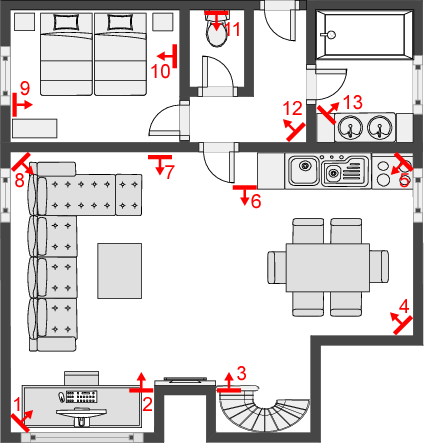
\includegraphics[scale=0.35]{img/SINS_database_floor_map.png}
	\caption[SINS database recording environment map]{SINS database recording environment map \footnotemark}
	\label{fig:sins-database-floor-map}
\end{figure}
\footnotetext{\href{https://bit.ly/2WPhYbS}{\nolinkurl{https://bit.ly/2WPhYbS}}}
\noindent
One person lived in the environment for a continuous duration of one week. In order to have an as realistic as possible data recording, there was no predefined set of scenarios. Due to that, the recorded activities also included being absent from the home. Although there were no restrictions on the actions, the number of activities that were labelled was limited, as indicated in table \ref{tab:sins-database-recorded-activities} of the appendix \ref{app:SINS-Database-Table}. In total there are 16 different recorded activities in five different rooms. Table \ref{tab:sins-database-recorded-activities}, which can be found in the appendix \ref{app:SINS-Database-Table}, lists the different activities along with the number of examples and the mean and standard deviation and the duration of all examples for each room.

\subsection[DCASE 2018 challenge - task 5 dataset]{DCASE 2018 challenge - task 5: monitoring of domestic activities based on multi-channel acoustics \footfullcite{dekkers_dcase_2018}}
\label{sub:DCASE-Task-Dataset}
This subsection contains all the necessary information about the challenge from the IEEE AASP Challenge on \gls{DCASE} 2018. The challenge finished in 2018, and the results, as well as the full dataset, were published. The main goal of the challenge was to classify multi-channel audio segments into predefined classes and determine how beneficial multi-channel recordings are for classification. 

\begin{figure}[htbp]
	\centering
	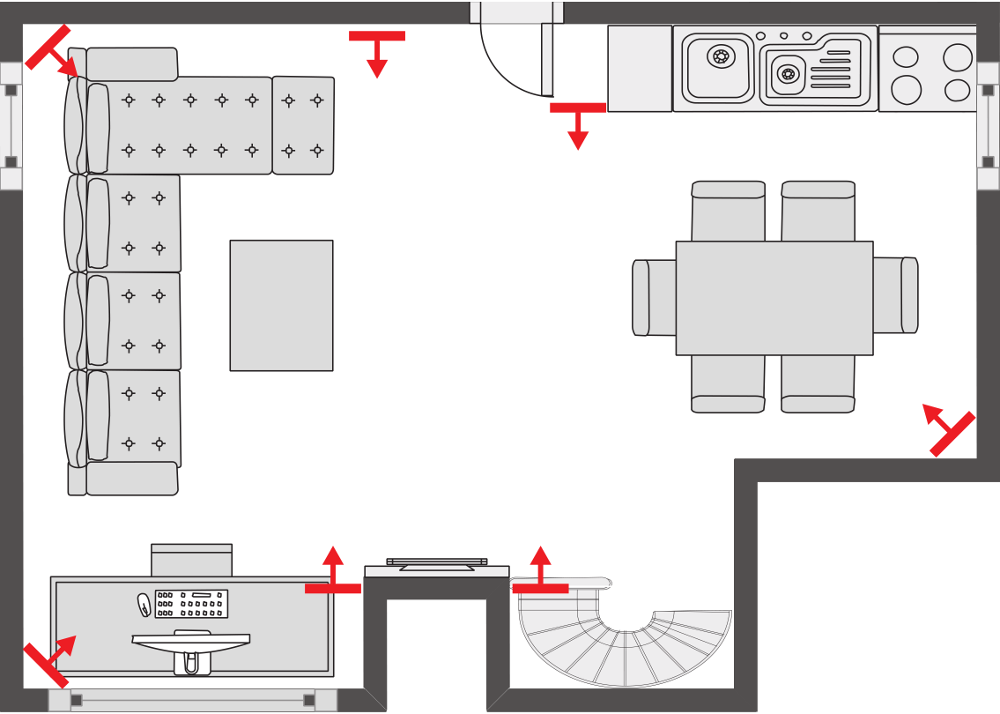
\includegraphics[scale=0.8]{img/DCASE_floor_map.png}
	\caption[2D floor plan of the combined kitchen and living room from DCASE]{2D floor plan of the combined kitchen and living room with the used sensor nodes \footnotemark}
	\label{fig:dcase-recordings-floor-plan}
\end{figure}
\footnotetext{\href{http://dcase.community/challenge2018/task-monitoring-domestic-activities}{\nolinkurl{dcase.community/challenge2018/task-monitoring-domestic-activities}}}
\noindent
The dataset used in the challenge is an abbreviation of the \nameref{sub:SINS-Database}; where only seven of the thirteen microphone nodes were considered. These nodes are from the room combination of the living room and the kitchen, as illustrated in figure \ref{fig:dcase-recordings-floor-plan}. Every recording of an activity is split into ten-second recordings, which are called segments. Every segment has four channels which correspond to the four different microphone channels of each node. Within the dataset, there are no overlapping sounds, from actions performed simultaneously. That means that every segment has an activity label assigned to it. There are a total of nine different activity labels, which all refer to a daily activity performed at home. Table \ref{tab:DCASE-activiies-performed} shows the activities performed in the dataset as well as the amount of 10 second segments and sessions of the activity.
\newline
\newline
In the challenge, the data was split into a development and an evaluation set. The development set is used for training the model and was made available for everyone participating in the challenge. It contains four of the seven microphone nodes which are 200h of audio data. This dataset also contains the corresponding label to each audio segment. The evaluation set is used for evaluating the final models to see their performance on never seen before data from the other three nodes. A session of an activity is a full recording of an action. Within both of these datasets, each session was kept together.
\begin{table}[htbp]
    \centering
    \caption[Activities performed in the dataset proposed by DCASE]{Activities performed in the dataset proposed by DCASE \footnotemark}
	\label{tab:DCASE-activiies-performed}
    \begin{tabular}{l|l|l}
        \toprule
        \textbf{Activity performed} & \textbf{\# 10s segments} & \textbf{\# sessions} \\ 
        \midrule[1pt]
        Absence (nobody present in the room) & 18860 & 42 \\
        \hline
        Cooking & 5124 & 13 \\ 
        \hline
        Dish washing & 1424 & 10 \\ 
        \hline
        Eating & 2308 & 13 \\ 
        \hline
        Other (present, but not doing any relevant activity) & 2060 & 118 \\ 
        \hline
        Social activity (visit, phone call, ...) & 4944 & 21 \\ 
        \hline
        Vacuum cleaning & 972 & 9 \\ 
        \hline
        Watching TV & 18648 & 9 \\ 
        \hline
        Working (typing, mouse clicking, ...) & 18644 & 33 \\ 
        \midrule[1pt]
        \textbf{Total} & \textbf{72984} & \textbf{268} \\
        \bottomrule
    \end{tabular}
\end{table}
\footnotetext{\href{http://dcase.community/challenge2018/task-monitoring-domestic-activities}{\nolinkurl{dcase.community/challenge2018/task-monitoring-domestic-activities}}}

\subsection{Music dataset}
\label{sub:Music-Dataset}

The second dataset used within the thesis is the music, which consists of songs classified by their respective genre. The songs are classified by the genre, according to \href{http://beatport.com}{beatport.com}, which is an electronic music-oriented online music store. Beatport is oriented primarily towards DJs, selling full songs as well as resources which can be used for remixes. Each genre consists of 30 different songs, which vary heavily in length, from 3min up to 10min. The dataset contains approximately 18 hours of music provided as a single channel mp3 files. Table \ref{tab:Music-Dataset} shows the genres from the dataset along with the number of songs within each.

\begin{table}[htbp]
    \centering
    \caption{Music genres in the music dataset along with the number of songs}
	\label{tab:Music-Dataset}
    \begin{tabular}{p{.70\textwidth} | p{.20\textwidth}}
        \toprule
        \textbf{Music genres} & \textbf{\# songs} \\ 
        \midrule[1pt]
        Deep House & 30 \\
        \hline
        Electronica Downtempo & 30 \\ 
        \hline
        Indie Dance & 30 \\ 
        \hline
        Melodic House and Techno & 30 \\ 
        \hline
        Techno Peak Time Driving Hard & 30 \\ 
        \hline
        Techno Raw Deep Hypnotic & 30 \\ 
        \hline
        Trance & 30 \\
        \midrule[1pt]
        \textbf{Total} & \textbf{210} \\
        \bottomrule
    \end{tabular}
\end{table}

\section{State of the art}
\label{sec:State-of-art}
Within this section of the thesis, two state-of-the-art concepts are introduced, which will be essential for the following chapters and used throughout the whole project. Therefore it is essential to be familiar with the terms, definitions and equations of triplet loss (\ref{sub:Triplet-Loss}) and Tile2Vec (\ref{sub:Tile2Vec}). First triplet loss (\ref{sub:Triplet-Loss}) will be introduced, and after that, the Tile2Vec (\ref{sub:Tile2Vec}) concept, which is an application of the triplet loss (\ref{sub:Triplet-Loss}).

\subsection{Triplet loss}
\label{sub:Triplet-Loss}
Triplet loss was first introduced in the field of face recognition by the paper (\cite{schroff_facenet_2015}) from Google. They describe a new approach to train face embeddings using online triplet mining.
\begin{figure}[htbp]
	\centering
	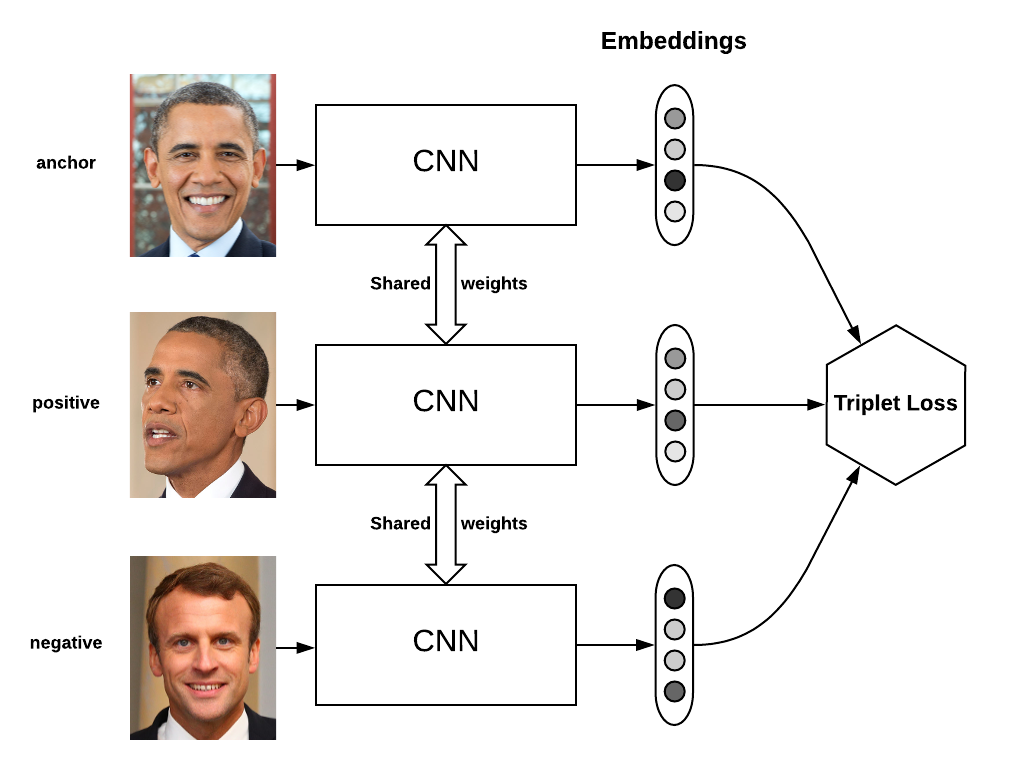
\includegraphics[scale=0.35]{img/Triplet_Loss_Architecture.png}
	\caption[Triplet Loss architecture visualisation]{Triplet Loss architecture visualisation \footnotemark}
	\label{fig:Triplet-Loss-Architecture}
\end{figure}
\footnotetext{\url{https://omoindrot.github.io/triplet-loss}}
\noindent
\myequations{Euclidean distance}
\begin{equation}
    \centering
    \begin{gathered}
        d(p,q) = \big|\big|q-p\big|\big|_2 = \sqrt{(q_1 - p_1)^2 + \dots + (q_n - p_n)^2} = \sqrt{\sum_{i=1}^n (q_i - p_i)^2}
    \end{gathered}
    \label{eq:Euclidean-Distance}
\end{equation}
\noindent
The introduced architecture helps to learn distributed embeddings by the notion of similarity and dissimilarity. Within the neural network architecture, multiple parallel networks are trained, which share the same weights among each other; this is illustrated in figure \ref{fig:Triplet-Loss-Architecture}. The objective is to build triplets consisting of an anchor $x_a$, a positive $x_p$ and a negative sample $x_n$. Where the positive sample is similar to the anchor and the negative one is dissimilar to the anchor. In the high dimensional vector space, contextually similar data points are projected in the near-by region ($x_a$ and $x_p$). In contrast, different data points are projected far away from each other ($x_a$ and $x_n$). This condition is defined by the equation \ref{eq:Triplet-Loss-Constraint}. Where $|| \cdot ||_2$ is defined as the euclidean distance with equation \ref{eq:Euclidean-Distance} and $\tau$ is the set of all possible triplets in the dataset.
\myequations{Triplet Loss constraint}
\begin{equation}
    \centering
    \begin{gathered}
        \Big|\Big|f_\theta(x_a) - f_\theta(x_p)\Big|\Big|_2^2 + \alpha < \Big|\Big|f_\theta(x_a) - f_\theta(x_n)\Big|\Big|_2^2 \\[10pt]
        \forall \big(f_\theta(x_a), f_\theta(x_p), f_\theta(x_n)\big) \in \tau
    \end{gathered}
    \label{eq:Triplet-Loss-Constraint}
\end{equation}
The embedding of a given sample $x$ is represented by $f_\theta(x) \in \mathbb{R}^d$, where $f$ is a some kind of network (e.g. fully connected \gls{NN}, \gls{CNN}, \gls{RNN}, or any other) with weights $\theta$. It embeds a sample $x$ into a $d$-dimensional Euclidean space. The loss, which will be minimised, is defined by the equation \ref{eq:Triplet-Loss}. Where $\alpha$ is a margin that is enforced between positive and negative pairs, it further puts a limit on how far the network can push the negative sample away to improve the loss. In equation \ref{eq:Triplet-Loss}, the notation $[\cdot]_+$ is used to represent the rectifier $\text{max}(0, \cdot)$.
\myequations{Triplet Loss function}
\begin{equation}
    \centering
    \mathcal{L} = \Bigg [\Big|\Big|f_\theta(x_a) - f_\theta(x_p)\Big|\Big|_2^2 - \Big|\Big|f_\theta(x_a) - f_\theta(x_n)\Big|\Big|_2^2 + \alpha \Bigg]_+
    \label{eq:Triplet-Loss}
\end{equation}
When the loss is minimised, it pushes the distance between $f_\theta(x_a)$ and $f_\theta(x_p)$ near zero. Contrarily it forces the distance between $f_\theta(x_a)$ and $f_\theta(x_n)$ to be higher than the distance between $f_\theta(x_a)$ and $f_\theta(x_p)$ plus some margin $\alpha$.
\newline
\newline
Generating all possible triplets of a dataset would result in many triplets which easily satisfy the equation \ref{eq:Triplet-Loss-Constraint}. These easy triplets would not contribute to the training and result in slower convergence, as they would still be passed through the network. Therefore it is crucial to select only hard triplets, which can enhance the model. This means that given $x_a$, $x_p$ is selected to be a hard positive such that equation \ref{eq:Triplet-Loss-Hard-Positive} is satisfied. Similarly, $x_n$ is a hard negative when equation \ref{eq:Triplet-Loss-Hard-Negative} is fulfilled. However, it is probably not feasible to make these calculations for the whole dataset, because they are computing-intensive. Nevertheless, it can be used to improve the model, for example, to better distinguish between classes which are quite similar.
\myequations{Triplet Loss hard positive}
\begin{equation}
    \centering
    \text{hard positive} = \text{argmax}_{x_p} \ \Big|\Big|f_\theta(x_a) - f_\theta(x_p)\Big|\Big|_2^2
    \label{eq:Triplet-Loss-Hard-Positive}
\end{equation}
\myequations{Triplet Loss hard negative}
\begin{equation}
    \centering
    \text{hard negative} = \text{argmin}_{x_n} \ \Big|\Big|f_\theta(x_a) - f_\theta(x_n)\Big|\Big|_2^2
    \label{eq:Triplet-Loss-Hard-Negative}
\end{equation}

\subsection{Tile2Vec}
\label{sub:Tile2Vec}
Tile2Vec was first introduced by the paper (\cite{jean_tile2vec_2018}) from Stanford University. It is an unsupervised representation learning algorithm that extends the distributional hypothesis from natural language to spatially distributed data. This hypothesis implies that words appearing in similar contexts tend to have similar meanings. Tile2Vec is used to learn compressed yet informative representations from unlabeled remote sensing data.
\newline
\newline
In the cited paper, the main focus is on remote sensing, which is the measurement of the Earth's surface through aircraft- or satellite-based sensors. In remote sensing, the biggest problem is the scarcity of labelled data. Thus the use of unsupervised machine learning is necessary. Hereafter the data, which is used to train the algorithm, consists of geospatial tiles.
\newline
\newline
The distributional hypothesis in linguistics is the idea that \flqq a word is characterised by the company it keeps\frqq. In \gls{NLP}, algorithms like Word2Vec and GloVe leverage this assumption to learn continuous representations that capture the nuanced meanings of vast word vocabularies.
\newline
\newline
Tile2Vec proposes to learn the representations on the level of remote sensing tiles, a generalisation of image patches to multi-spectral data. The context of each tile relies on the spatial neighbourhood, which is defined as some distance in the geographic space. The assumption is that tiles which are located close together have a similar meaning and should, therefore, have similar representations in the embedding space.
\newline
\newline
To learn a mapping from image tiles to low-dimensional embeddings, a \gls{CNN} is trained on triplets of tiles, where each triplet consists of an anchor tile $x_a$, an adjacent tile $x_p$ which is geographically close and a distant tile $x_n$ which is farther away. Following the distributional assumption, the Euclidean distance (eq. \ref{eq:Euclidean-Distance}) between the embedding of the anchor tile and the neighbour tile is minimised, while maximising the distance between the anchor and distant embedding (\ref{sub:Triplet-Loss}). For each tile triplet $(x_a, x_p, x_n)$ the triplet loss (\ref{eq:Triplet-Loss}) is therefore minimized.
\newline
\newline
But when $||f_\theta(x_a) - f_\theta(x_p)||_2 < ||f_\theta(x_a) - f_\theta(x_n)||_2$, all embeddings can be scaled by some constant in order to satisfy the margin and bring the loss to zero. After a small number of iterations, the \gls{CNN} learns to increase the embedding magnitudes to decrease the loss to zero. By penalising the embeddings $l^2$-norms, the network is forced to generate embeddings within a hypersphere, leading to a representation space in which relative distances have meaning. The regularisation term is defined by $\lambda \Big(||f_\theta(x_a^{(i)})||_2 + ||f_\theta(x_p^{(i)})||_2 + ||f_\theta(x_n^{(i)})||_2\Big)$, which can be controlled using the hyperparameter $\lambda$. The cost function of the Tile2Vec algorithm is defined by equation \ref{eq:Tile2Vec-Cost-Function}. Where $N$ is the cardinality of the valid triplets in the dataset and $\mathcal{L}$ is the triplet loss (\ref{eq:Triplet-Loss}).
\myequations{Tile2Vec Cost function}
\begin{equation}
    \centering
    \min_\theta \sum_{i=1}^N \Bigg[\mathcal{L}\Big(x_a^{(i)}, x_p^{(i)}, x_n^{(i)}, \theta\Big) + \lambda \Big(||f_\theta(x_a^{(i)})||_2 + ||f_\theta(x_p^{(i)})||_2 + ||f_\theta(x_n^{(i)})||_2\Big)\Bigg]
    \label{eq:Tile2Vec-Cost-Function}
\end{equation}
The sampling procedure for the triplet $(x_a, x_p, x_n)$ is described by two parameters, the tile size and the neighbourhood radius. The tile size defines the pixel width and height of a single tile. The neighbourhood radius defines the region around the anchor tile from which to sample the adjacent tile. The centre of the neighbour tile must be within this radius of the anchor, and the distant tile is then sampled at random from outside the radius.

\section{Status in relation to project}
\label{sec:Status-Relation-Project}
This section of the chapter focuses on the current state of the art deep learning techniques for audio signal processing, which are relevant for this project. Many of these techniques were first introduced for the field of image processing and then adapted for audio processing. However, there is a vast difference between image and audio data, for example, raw audio data samples from a one-dimensional time-series signal, whereas image data is two-dimensional. Thus many of the traditional techniques had to be adapted for audio data.
\newline
\newline
This thesis considers its main task to be a \textit{sequence classification}, where a single global class label needs to be predicted for an audio sequence. However, there is no defined terminology for deep learning with audio. Thus there are many variant terms in use.
\newline
\newline
Mel spectrogram (\ref{sub:Mel-Spectrogram}) is the most common representation used in traditional audio signal processing, log-mel spectrograms are the dominant feature in deep learning, followed by raw waveforms or complex spectrograms. Raw waveforms avoid hand-designed features, which should allow better to exploit the improved modelling capability of deep learning models. However, this incurs higher computational costs and data requirements, and the benefits are hard to realize in practice. For \gls{ASR}, log-mel spectrograms provide a more compact representation, and methods using these features usually need fewer data and training to achieve results, which are comparable in performance to a setup where raw audio is used. \glspl{MFCC} and log-mel spectrograms are gladly used because they were inspired by the human auditory system, which makes the use of these features reasonable.
\newline
\newline
Across many audio processing domains, \glspl{CNN}, \glspl{RNN} and \glspl{CRNN} are employed successfully, with no clear preference. All three can model temporal sequences, solve sequence classification and many more applications. \glspl{CNN} have a fixed receptive field, which limits the temporal context taken into account for a prediction, but at the same time makes it very easy to widen or narrow the context used. The receptive field can be increased using larger kernels or stacking more layer. Alternatively, another way to increase the receptive field of a \gls{CNN} is to stack dilated convolution layers (\ref{subsub:Dilated-Convolution}), which apply the convolution filter over an area larger than its filter length. These convolutions obtain a vast receptive field with just a few layers while preserving the input resolution as well as computational efficiency (\cite{franceschi_unsupervised_2020}).
\newline
\newline
\glspl{RNN} can, theoretically, base their predictions on an unlimited temporal context, but first need to learn to do so, which may require adaptions to the model (such as gated recurrent units \ref{sub:Gated-Recurrent-Unit}). Furthermore, they require processing the input sequentially, making them slower to train and to evaluate than \glspl{CNN}. \Glspl{CRNN} offer a compromise in between, inheriting both \glspl{CNN} and \glspl{RNN} advantages and disadvantages.
\newline
\newline
Thus the process of choosing the superior model for a specific task is still an open research question. From existing literature, this is very hard to answer, since the different research groups yield state-of-the-art results with different models. This may be due to each research group’s specialized informal knowledge about how to design and tune a particular architecture type effectively.\footnote{\fullcite{purwins_deep_2019}}
\newline
\newline
With the possible exception of speech recognition, in the industry, for the most popular languages, all tasks in all audio domains face relatively small datasets, posing a limit on the size and complexity of deep learning models trained on them. However, in other domains, such as computer vision the shortage of labelled data for a particular task is offset by the widespread availability of models trained on the ImageNet dataset. Nevertheless, no comparable task and dataset exist for the audio domain.
\newline
\newline
Most of the models submitted in the \fullref{sub:DCASE-Task-Dataset} used \glspl{MFCC} or log-mel spectrograms as acoustic features along side with a \gls{CNN} as their main architecture. The winner of the challenge was the IBM research team, which show their model in the paper (\cite{inoue_domestic_2018}). They only used the input data provided in the dataset, from the challenge, and sampled it at a rate of 16kHz. From the dataset, the log-mel energies (\ref{sub:Mel-Spectrogram}) are extracted and used to train a \gls{CNN}. They propose data augmentation techniques using shuffling and mixing two sounds in the same class, to mitigate the unbalanced training dataset. Which led them to train their model on a much larger dataset than the rest.
\newline
\newline
Another model in the challenge, proposed in the paper (\cite{liu_ensemble_2018}), uses an ensemble of a \gls{CNN} and a \gls{RNN} to achieve some remarkable results without any data augmentation. 